\section{Verification and Validation}

\subsection{Terminology}

There are some differences between the terms verification and validation.

\highspace
First of all, the verification is internal. Despite the validation is external. Assuming an abstract process with the following levels:

\begin{figure}[!htp]
    \centering
    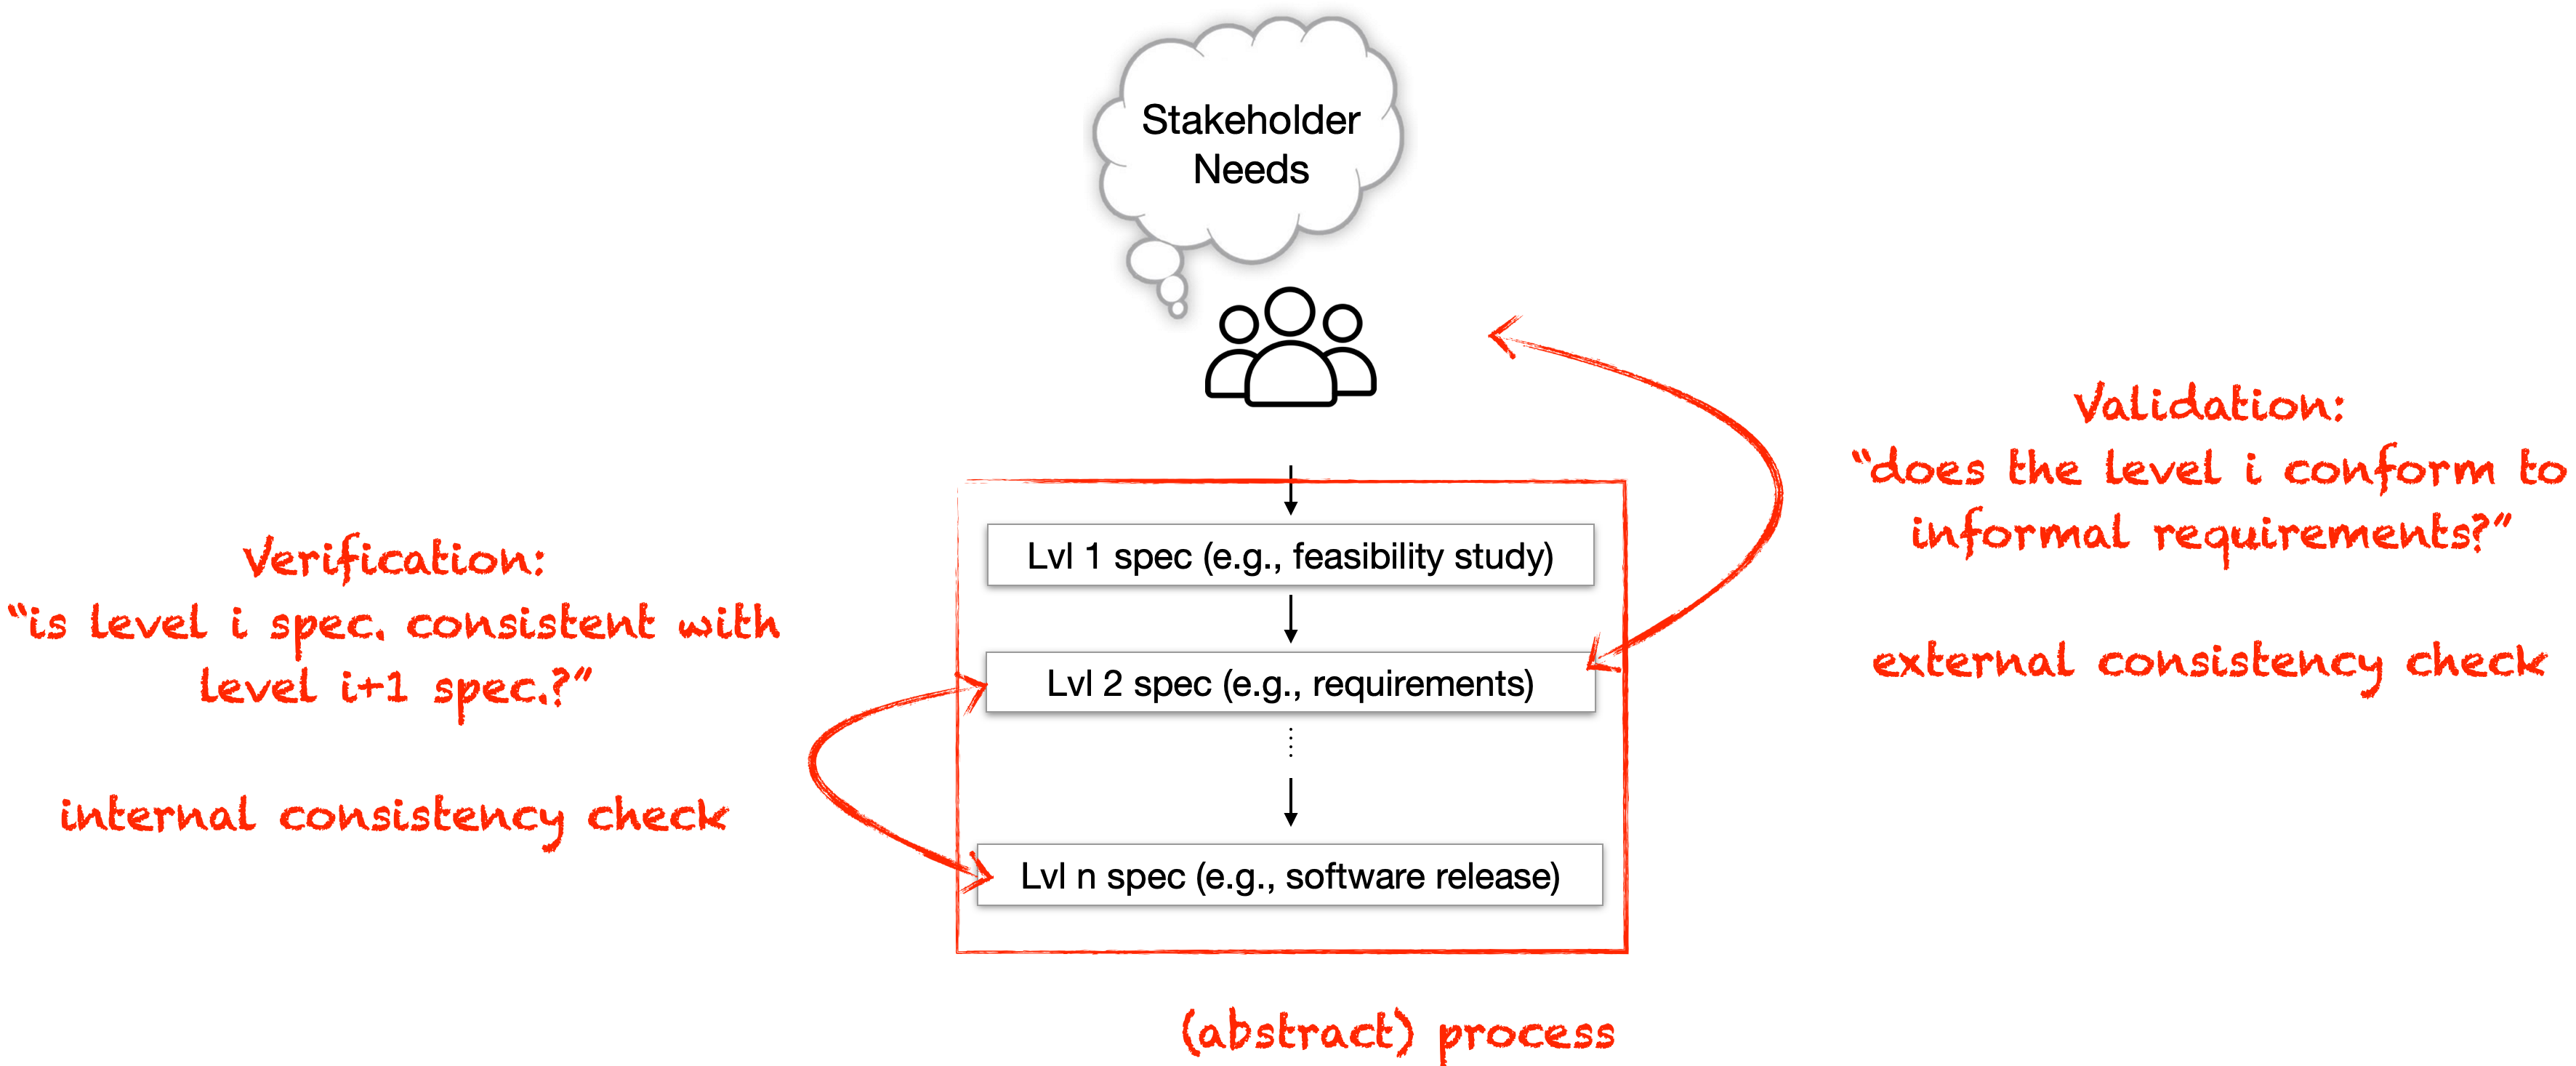
\includegraphics[width=\textwidth]{img/verification-and-validation-1.png}
\end{figure}

\noindent
The \textbf{verification} is intended as: \dquotes{Is level i consistent with level $i+1$?}. It's an \textbf{internal consistency check}. The \textbf{validation} is: \dquotes{Does level i conform to needs?}. It's an \textbf{external consistency check}.

\highspace
\href{https://en.wikipedia.org/wiki/A_Guide_to_the_Project_Management_Body_of_Knowledge}{The PMBOK guide}, also adopted by the \href{https://en.wikipedia.org/wiki/IEEE}{IEEE} as a standard, defines them as follows in its 4th edition:
\begin{itemize}
    \item \definition{Validation}. The assurance that a \textbf{product}, \textbf{service}, or \textbf{system} \textbf{meets the needs of the customer and other identified stakeholders}. It often involves acceptance and suitability with external customers. Contrast with verification.
    
    \item \definition{Verification}. The \textbf{evaluation of whether or not a product}, \textbf{service}, or \textbf{system complies with a regulation}, \textbf{requirement}, \textbf{specification}, or \textbf{imposed condition}. It is often an internal process. Contrast with validation.
\end{itemize}

\highspace
Another fundamental topic when we speak about verification and validation is \definition{Quality Assurance (QA)}. It \textbf{defines the policies and processes to achieve quality}. So it can \textbf{judge the quality and find defects}. 

A direct \textbf{consequence} of the QA is the \textbf{improvement of the quality}. With the term \dquotes{quality}, we refer to an ideal absence of defects (impossible) and an absence of other issues that prevent the fulfilment of non-functional requirements or the degradation of some software qualities.

\highspace
Since it is impossible to have zero defects, a \textbf{periodic quality assurance evaluation is critical}. Ideally, every artefact shall be the subject of QA; even the verification artefacts must be verified!

\newpage

\noindent
The \definition{V-model} is a \textbf{graphical representation of a systems development lifecycle}. It is used to produce rigorous development lifecycle models and project management models. It describes the activities and the results that must be made during product development.

\begin{figure}[!htp]
    \centering
    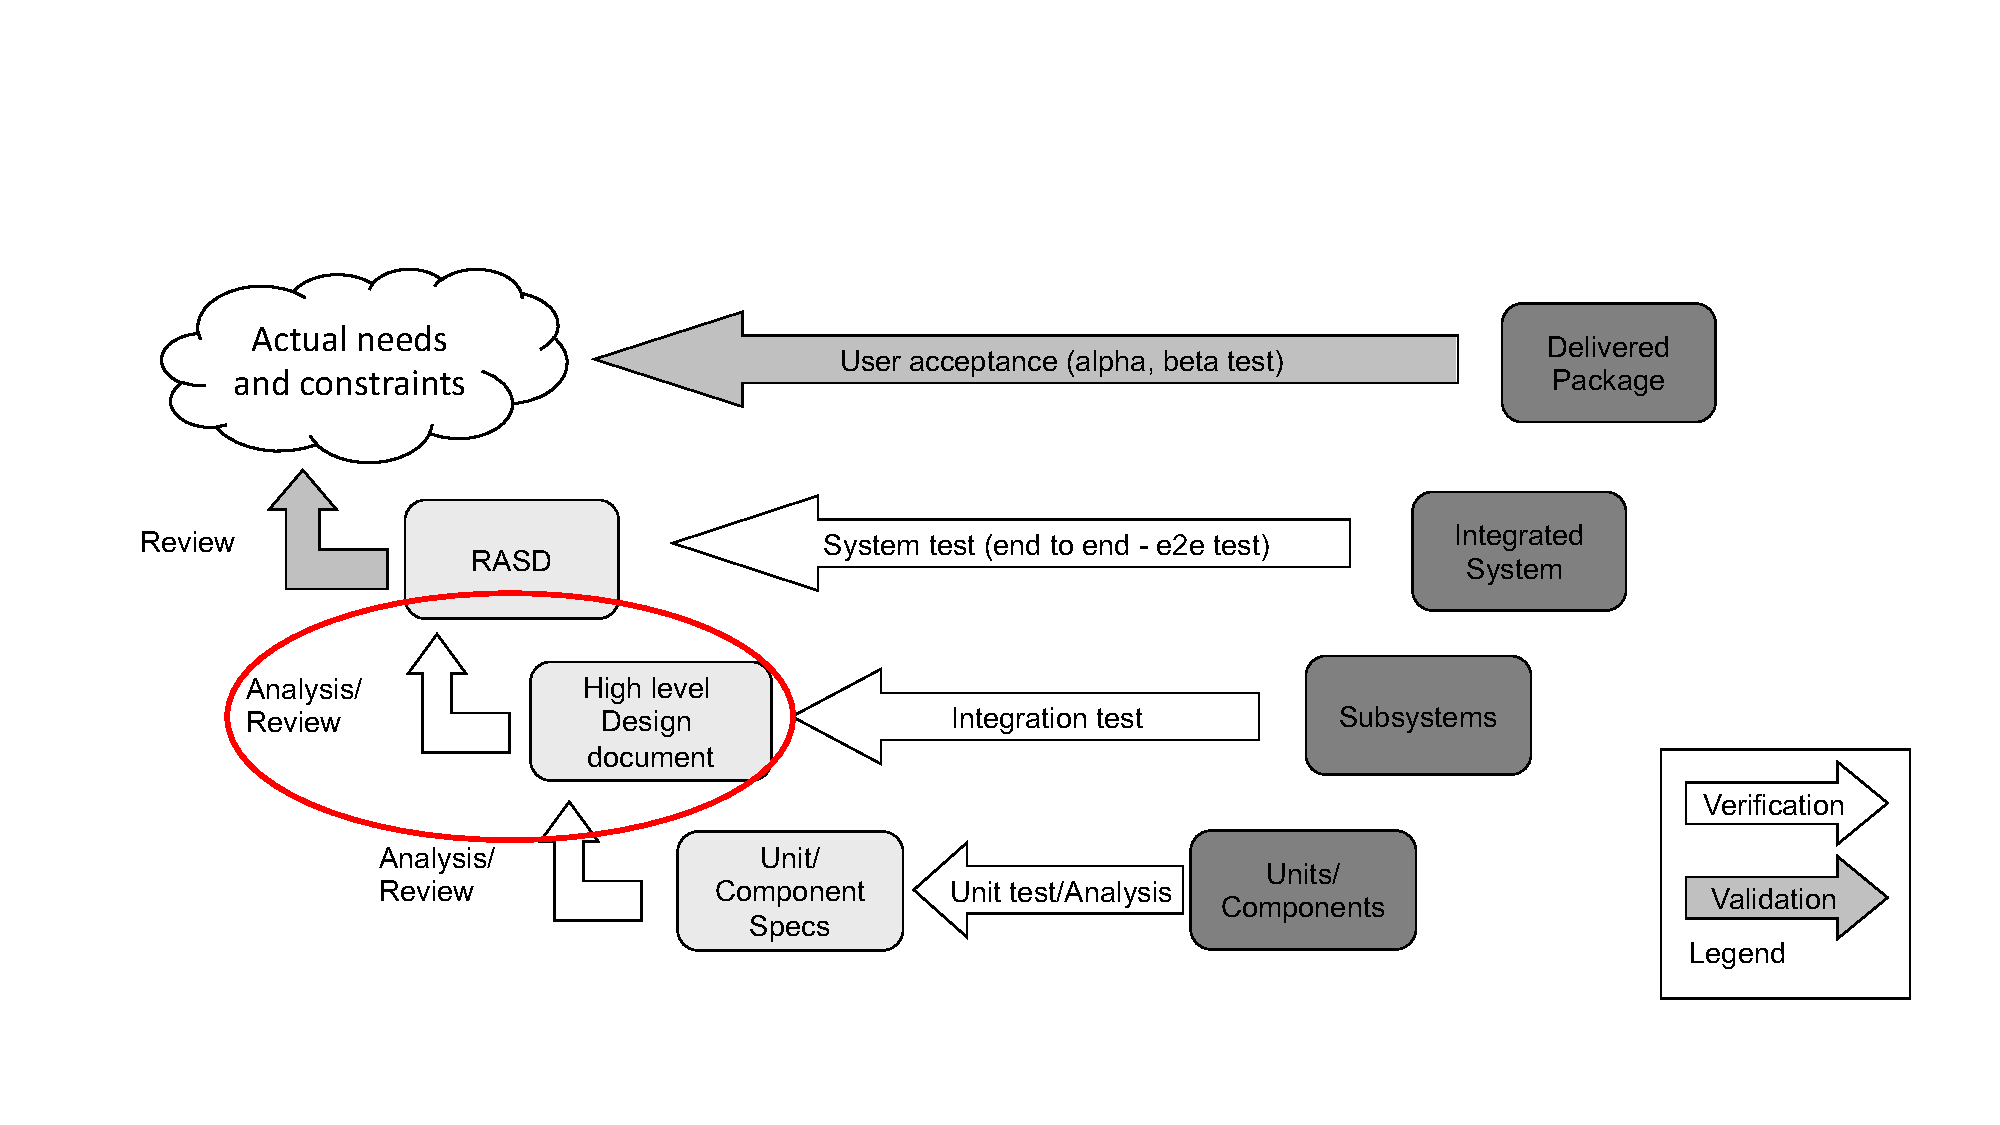
\includegraphics[width=\textwidth]{img/v-model-1.pdf}
    \caption{The V-model; verification is emphasized on the left.}
\end{figure}

\noindent
The \emph{left side} of the \dquotes{V} represents the decomposition of requirements and the creation of system specifications. The \emph{right side} of the \dquotes{V} represents an integration of parts and their validation.

\highspace
We have presented the V-model to help you understand where the verification can be placed.

\highspace
Now, the \textbf{verification} is concerned with the code and the architecture. Considering the \textbf{software} side, it has two possible approaches:
\begin{itemize}
    \item \definition{Static Analysis}. It is \textbf{done using source code or other software artefacts but \emph{without execution}}. Note that the analysis is static, but the properties are dynamic.

    \item \definition{Dynamic Analysis (Testing)}. It is \textbf{done by executing the sources}. The analysis is made by \textbf{comparing} the actual behaviour and the expected one.
\end{itemize}
On the other hand, to verify the \textbf{architectural level}, it is necessary to consider some aspects:
\begin{itemize}
    \item The \textbf{structure must be consistent}. Some \example{examples}:
    \begin{itemize}
        \item For every required interface, a corresponding provided interface exists.
        
        \item Sequence diagrams are consistent with component diagrams and with the defined interfaces.
        
        \item Each component has one or more modules that implement it.
    \end{itemize}

    \item All \textbf{functional requirements must have the possibility to be satisfied}. Some \example{examples}:
    \begin{itemize}
        \item Each requirement is mapped on one or more components.
        
        \item Each use case event flow is detailed in terms of one or more sequence diagrams.
    \end{itemize}

    \item \textbf{Concurrent use of resources must be correctly defined}. Problems like order violation or a deadlock are expected. Some techniques must be applied to analyze these problems. 
    
    \item \textbf{Non-functional requirements must have the possibility to be fulfilled}.
\end{itemize}